\chapter{Clustering}
\label{ch:capitolo2}

This chapter of the report aims at illustrating the clustering analysis performed on the dataset at hand.
The employed clustering techniques are K-means (Centroid-based), DBSCAN (density-based) and hierarchical clustering.

The analysis conducted using these methods focused only exclusively on the dataset's numerical attributes, which were appropriately log-transformed (as mentioned in the \textit{Variable Transformation} section) and normalized using \texttt{MinMaxScaler}.  
For the K-means algorithm, \texttt{totalNominations} and \texttt{totalMedia} were excluded due to their high proportion of zero values, which negatively affected cluster formation.

In addition, an attempt was made to incorporate categorical variables to the analysis with the K-means algorithm by converting them into binary attributes and constructing a mixed-distances matrix. 
Distances were then calculated using the Euclidean distance for numerical (log-tranformed and scaled) features and the Jaccard similarity for binary ones. 
However, this approach was computationally expensive and did not lead to any improvement in the results.

\textbf{RIVEDERE PARTE PCA}
Principal Component Analysis (PCA) was applied to the preprocessed data just for clusters visualization purposes. 
Analysis of the numerical attributes reveals that 4 principal components are optimal when excluding variables with many zero values, while 5 components are needed when including all variables. 
These numbers of components capture the maximum meaningful variance, as shown by the point in the plots where where the line starts to flatten, indicating that adding more components doesn't increase explained variance significantly. 
The plots in figure~\ref{fig:pca_diff} show the differences between these two approaches. \textbf{IN REALTA' NON SI VEDE TROPPO LA DIFFERENZA, QUINDI MAGARI NON FARE PCA MA SOLO VISUALIZZAZIONE CON ISTOGRAMMI??? oppure semplicemente tenere solo uno dei due plot?}
\begin{figure}[H]
    \centering
    \begin{subfigure}[b]{0.40\textwidth}
        \centering
        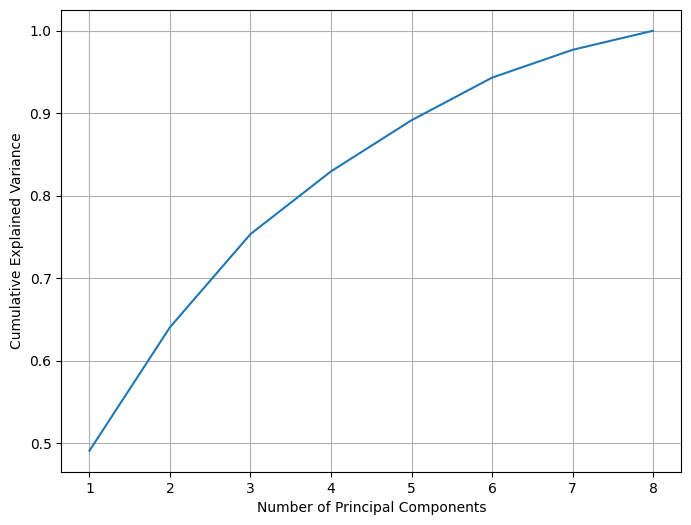
\includegraphics[width=\textwidth]{plots/pca_kmeans.png}
        \caption{PCA excluding variables}
        \label{fig:sse_silh_kmeans}
    \end{subfigure}
    \begin{subfigure}[b]{0.40\textwidth}
        \centering
        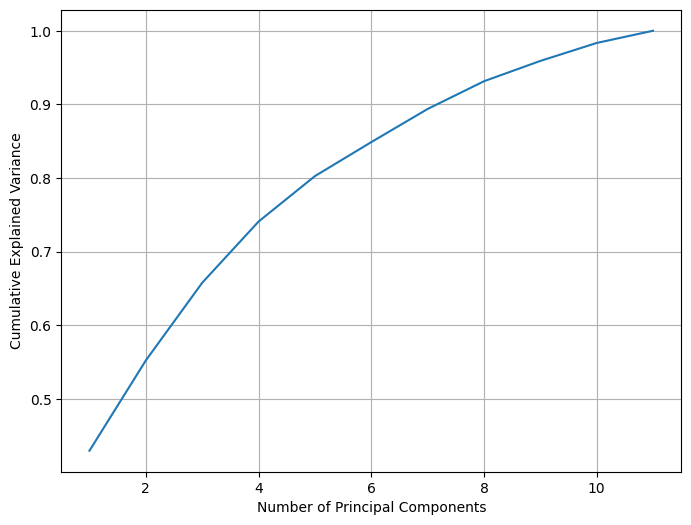
\includegraphics[width=\textwidth]{plots/pca5.png}
        \caption{PCA with all variables}
        \label{fig:pca5}
    \end{subfigure}
    \caption{Principal Component Analysis}
    \label{fig:pca_diff}
\end{figure}

\section{K-means}\label{sec:centroid_based}
%The clustering analysis performed with the K-means algorithm focused on the numeric variables of the dataset, excluding \texttt{awardWins}, \texttt{awardNominationsExcludeWins}, and \texttt{totalCredits} due to their high proportion of zero values, which negatively affected cluster formation. 
%The variables have been appropriately log-transformed (as illustrated in the \textit{Variable Transformation} section) and normalized with \texttt{StandardScaler}.

To identify the optimal number of clusters, both the SSE and Silhouette scores were computed. The goal was to find a configuration that minimizes the SSE while maintaining a robust Silhouette score and a proper \textit{k}. 
The plots in figure~\ref{fig:sse_silh_kmeans} demonstrate that \textit{k} = ??? provides the optimal balance between these metrics. Choosing \textit{k} = ??? returns a SSE score of ??? and Silhouette score of ???. 
\textbf{VALORI TROPPO ALTI, VEDERE SE CAMBIANO CAMBIANDO SCALING E/O TOGLIENDO OUTLIER}

% To visualize the clustering results, Principal Component Analysis (PCA) was employed. The plot in figure~\ref{fig:pca_kmeans} reveals that 4 principal components are enough to capture the optimal amount of variance for the selected variables, as evidenced by the the point where the line starts to flatten, indicating that adding more components doesn't increase explained variance significantly.
The cluster results are presented in figure~\ref{fig:pairplot_kmeans}. 

\begin{figure}[H]
    \centering
    \begin{subfigure}[b]{0.49\textwidth}
        \centering
        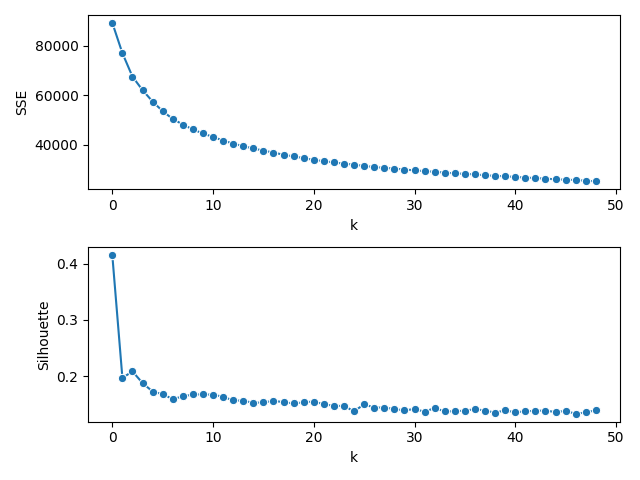
\includegraphics[width=\textwidth]{plots/sse_silh_kmeans.png}
        \caption{SSE and Silhouette scores}
        \label{fig:sse_silh_kmeans}
    \end{subfigure}
    % \hfill
    % \begin{subfigure}[b]{0.3\textwidth}
    %     \centering
    %     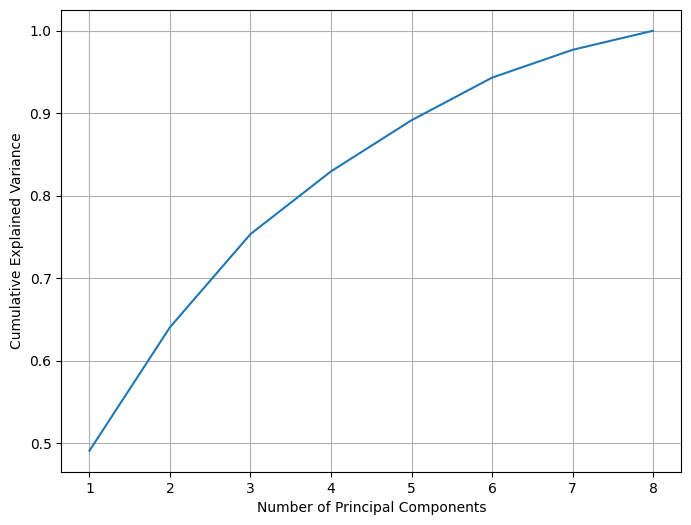
\includegraphics[width=\textwidth]{plots/pca_kmeans.png}
    %     \caption{PCA Analysis}
    %     \label{fig:pca_kmeans}
    % \end{subfigure}
    % \hfill
    \begin{subfigure}[b]{0.49\textwidth}
        \centering
        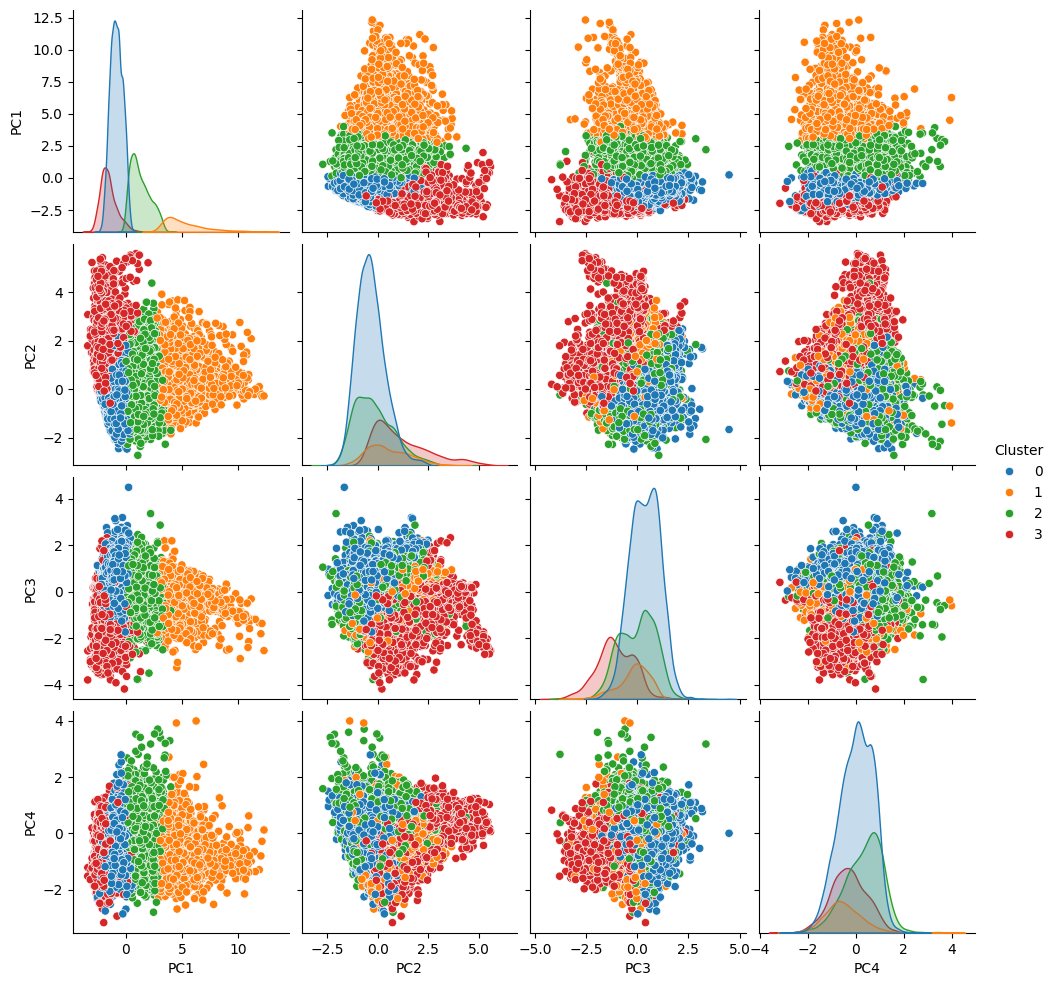
\includegraphics[width=\textwidth]{plots/pairplot_kmeans.png}
        \caption{K-means Visualization}
        \label{fig:pairplot_kmeans}
    \end{subfigure}
    \caption{K-means clustering analysis}
    \label{fig:three_subplots}
\end{figure}
The distribution of data points across the four clusters is as follows (shown in percentage of data points per cluster):
% Red (0): 51.68\%, Blue (1): 7.42\%, Green (2): 24.22\%, Orange (3): 16.68\%.
% The clusters are not as well-separated in most Principal Component combinations as they are with PC1. 
% In fact, in the other combinations, the clusters tend to overlap and their boundaries are not always clearly distinct.
% This might be an indication that the true clusters have irregular shapes or different densities, resulting in boundaries between them being not clearly defined.



\section{DBSCAN}\label{sec:density_based}
To determine the optimal DBSCAN parameters, the \textit{k\textsuperscript{th} nearest neighbors} method was used: this allows to identify \textit{eps} (the maximum distance between two points for them to be considered neighbors) given the value of \textit{Minpts} (minimum number of points in a neighborhood for a point to be considered a core point).
Initially, \textit{Minpts} was set to 22, following the rule of setting it above twice the number of dimensions. 
However, due to the dataset's unbalanced nature and the sparsity of high-dimensional data, reducing \textit{Minpts} to 11 allowed the formation of smaller clusters while preventing the risk of detecting only one dominant cluster and classifying many minority groups as noise instead of distinct clusters.
To determine \textit{eps}, the k\textsuperscript{th} nearest neighbors plot with \textit{k} = 11 was analyzed (figure ~\ref{fig:DBSCAN_kth_graph}). While the "knee" point suggested an eps of around 0.1, this value would have resulted in excessive noise and a single dominant cluster. 
To address this, eps was set to 1.564, allowing for meaningful connectivity while preserving the detection of smaller clusters without merging them into a single entity. 
The algorithm identified 4 groups in the dataset, including one representing noise (1,753 points). 
The largest cluster contains 13,198 points, while the smaller clusters consist of 733 and 747 points, 
respectively.The  results are shown in figure~\ref{fig:DBSCAN_provvisoria}

To conclude, by adjusting \textit{eps} and \textit{Minpts} appropriately, the clustering results achieved a Silhouette score of 0.139 \textbf{(SIL CONTANDO OUTLIERS)}, indicating little improved cluster separation and reduced noise, which is considered good enough for an unbalanced, high-dimensional dataset.

\begin{figure}[H]
    \centering
    \begin{subfigure}[b]{0.49\textwidth}
        \centering
        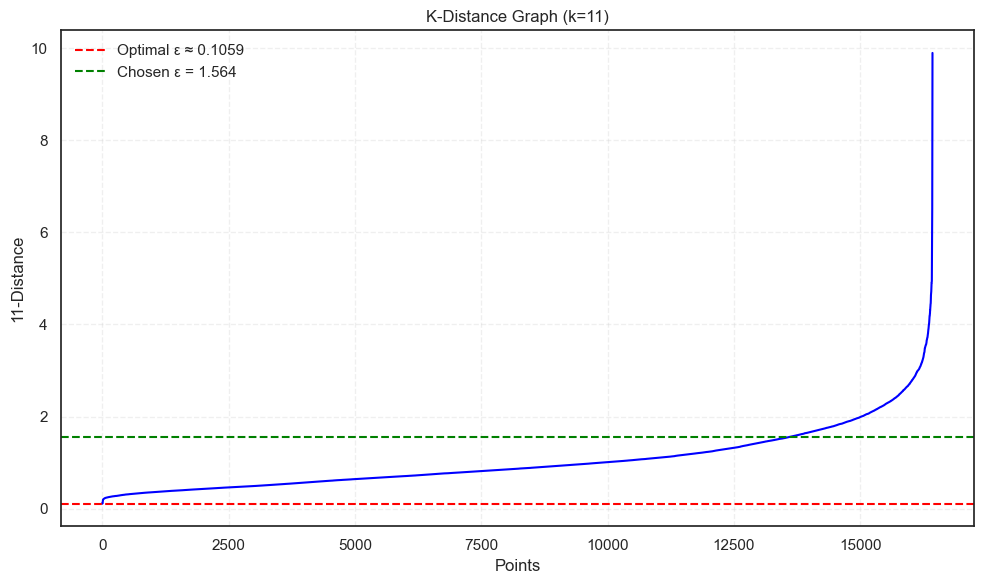
\includegraphics[width=\textwidth]{plots/DBSCAN_kth_graph.png}
        \caption{k\textsuperscript{th} nearest neighbors}
        \label{fig:DBSCAN_kth_graph}
    \end{subfigure}
    % \hfill
    % \begin{subfigure}[b]{0.3\textwidth}
    %     \centering
    %     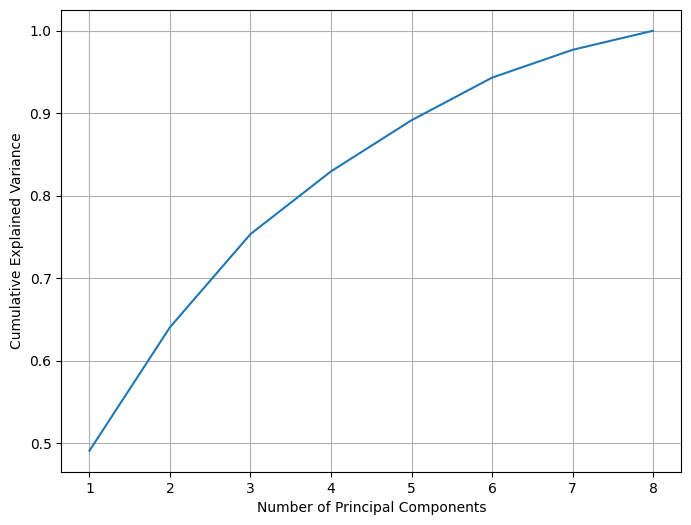
\includegraphics[width=\textwidth]{plots/pca_kmeans.png}
    %     \caption{PCA Analysis}
    %     \label{fig:pca_kmeans}
    % \end{subfigure}
    % \hfill
    \begin{subfigure}[b]{0.49\textwidth}
        \centering
        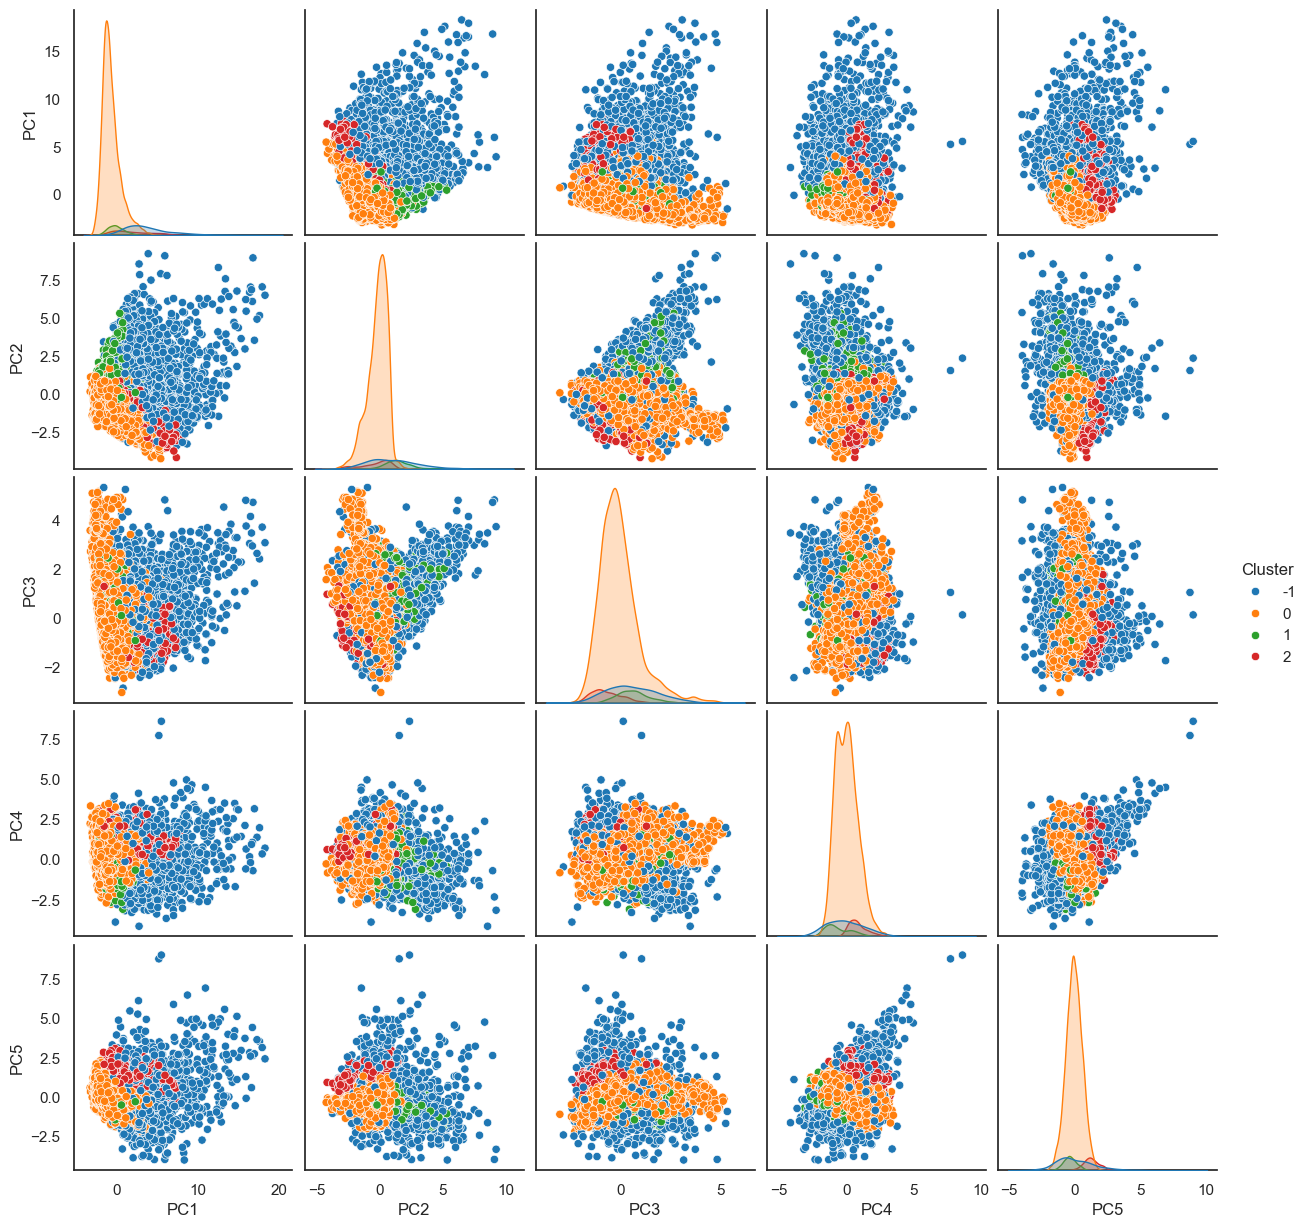
\includegraphics[width=\textwidth]{plots/DBSCAN_provvisoria.png}
        \caption{DBSCAN Visualization}
        \label{fig:DBSCAN_provvisoria}
    \end{subfigure}
    \caption{DBSCAN clustering analysis}
    \label{fig:three_subplots}
\end{figure}




\section{Hierarchical clustering}\label{sec:hierarchical}
Hierarchical clustering was performed using all linkages (Ward, Average, Complete, Single), with the Euclidean distance metric.
Figure~\ref{fig:hier_clust_stats} shows the results of the analysis, which includes the Silhouette and SSE scores, as well as the maximum and minimum percentage of points per cluster.
\begin{figure}[H]
    \centering

    % Left: Tall figure (a)
    \begin{subfigure}[t]{0.49\textwidth}
        \centering
        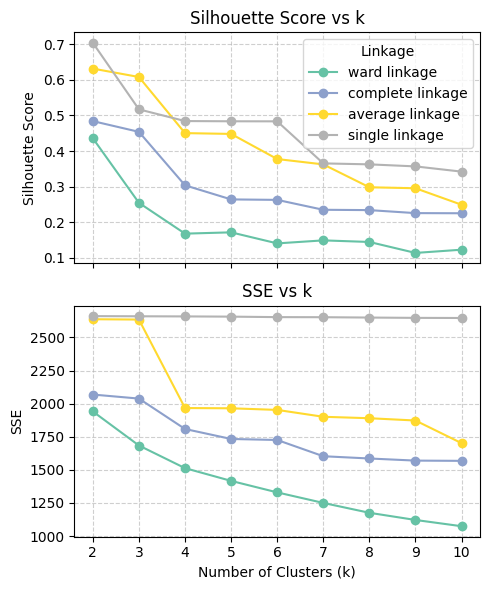
\includegraphics[width=0.95\textwidth]{plots/sil_sse_hierarchical_clust.png}
        \subcaption{Silhouette and SSE scores}
        \label{fig:sil_sse_hierarchical_clust}
    \end{subfigure}
    \hfill
    \begin{subfigure}[t]{0.49\textwidth}
        \centering
        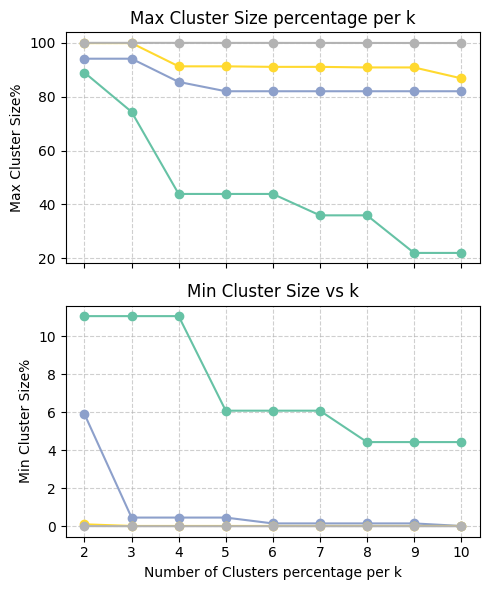
\includegraphics[width=0.95\textwidth]{plots/max_min_pctg.png}
        \subcaption{Max/Min percentage of points per cluster}
        \label{fig:max_min_pctg}
    \end{subfigure}
    \caption{Hierarchical clustering metrics for different numbers of clusters}
    \label{fig:hier_clust_stats}
\end{figure}

From figure~\ref{fig:max_min_pctg}, it can be observed that Single linkage produces a single cluster which contains basically all data points. This makes it unsuitable for this use case.
Average and Complete linkages produce a cluster with a high maximum cluster size (above 90\% of the dataset for all the number of clusters tested for Average, and 80\% for Complete).
These results are likely due to a few different causes: 
\begin{itemize}
    \item High density of points in a certain area of the feature space, which leads to the formation of large clusters;
    \item Presence of outliers (other than the ones that were removed), which can skew the clustering results by pulling the centroids towards them, resulting in larger clusters;
    \item High dimensionality of the dataset, which makes it more difficult to separate clusters effectively.
\end{itemize}

These issues are mitigated by Ward linkage, which produces less dominant biggest clusters for all numbers of clusters tested. The minimum cluster size is also consistently more balanced across different numbers of clusters.


\section{General considerations}\label{sec:considerations}